\documentclass[conference]{IEEEtran}
\usepackage{amsmath,amssymb}
\usepackage{graphicx}
\usepackage{booktabs}
\usepackage{cite}

\title{Graph Neural Networks for Protein Folding}
\author{\IEEEauthorblockN{Alice Anders}
\IEEEauthorblockA{Department of Biology\\
University of Example}
\and
\IEEEauthorblockN{Bob Baker}
\IEEEauthorblockA{Department of Computer Science\\
University of Example}}

\begin{document}
\maketitle

\begin{abstract}
Proteins fold into shapes that decide what they do. We treat a protein
as a graph of its residues and learn its structure by passing messages
along the graph. On a standard benchmark the model predicts contact maps
more accurately than sequence-only baselines.
\end{abstract}

\section{Introduction}
Predicting how a protein folds from its sequence is a central problem in
structural biology~\cite{jumper2021}. Each residue interacts with the
residues it touches, which makes a graph a natural description of the
structure~\cite{gilmer2017}.

\section{Method}
A graph neural network updates the state of each residue from the states
of its neighbours.

Fig.~\ref{fig:architecture} shows the architecture.

\begin{figure}[!htb]
  \centering
  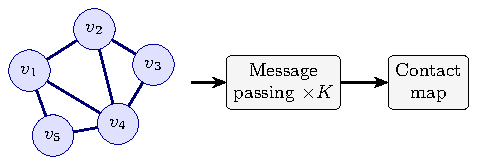
\includegraphics[width=\linewidth]{figures/architecture.pdf}
  \caption{The model: residues are nodes and contacts are edges.}
  \label{fig:architecture}
\end{figure}

\section{Results}
Table~\ref{tab:results} compares the model with two baselines
from~\cite{rao2021}.

\begin{table}[!htb]
  \centering
  \caption{Precision of contact prediction}
  \label{tab:results}
  \begin{tabular}{lcc}
    \toprule
    Model & Top-$L$ & Top-$L/5$ \\
    \midrule
    Sequence CNN & 0.41 & 0.63 \\
    Transformer & 0.52 & 0.74 \\
    Ours & \textbf{0.61} & \textbf{0.82} \\
    \bottomrule
  \end{tabular}
\end{table}

\bibliographystyle{IEEEtran}
\bibliography{refs}

\end{document}
